% !TEX root = ../multi_task.tex

We evaluate the presented MTL method on a number of problems. First, we use MultiMNIST \citep{multi_mnist}, an MTL adaptation of MNIST \citep{mnist}. Next, we tackle multi-label classification on the CelebA dataset \citep{celeba} by considering each label as a distinct binary classification task. These problems include both classification and regression, with the number of tasks ranging from 2 to 40. Finally, we experiment with scene understanding, jointly tackling the tasks of semantic segmentation, instance segmentation, and depth estimation on the Cityscapes dataset \citep{cityscapes}. We discuss each experiment separately in the following subsections.

The baselines we consider are (i) \textbf{uniform scaling:} minimizing a uniformly weighted sum of loss functions \mbox{$\frac{1}{T}\sum_t \lL^t$}, \mbox{(ii) \textbf{single task:}} solving tasks independently, \mbox{(iii) \textbf{grid search:}} exhaustively trying various values from $\{ c^t \in [0,1] | \sum_t c^t = 1\}$ and optimizing for $\frac{1}{T}\sum_t c^t \lL^t$, \mbox{(iv) \textbf{\citet{Kendall2018}:}} using the uncertainty weighting proposed by \citet{Kendall2018}, and \mbox{(v) \textbf{GradNorm:}} using the normalization proposed by \citet{Chen2018}.



\subsection{MultiMNIST}
\label{sec:multi_mnist_exp}

Our initial experiments are on MultiMNIST, an MTL version of the MNIST dataset \citep{multi_mnist}. In order to convert digit classification into a multi-task problem, \citet{multi_mnist} overlaid multiple images together. We use a similar construction. For each image, a different one is chosen uniformly in random. Then one of these images is put at the top-left and the other one is at the bottom-right. The resulting tasks are: classifying the digit on the top-left (task-L) and classifying the digit on the bottom-right (task-R). We use 60K examples and directly apply existing single-task MNIST models. The MultiMNIST dataset is illustrated in the supplement.

We use the LeNet architecture \citep{mnist}. We treat all layers except the last as the representation function $g$ and put two fully-connected layers as task-specific functions (see the supplement for details). We visualize the performance profile as a scatter plot of accuracies on task-L and task-R in Figure~\ref{fig:multi_mnist_performance_curve}, and list the results in Table~\ref{tab:multi_mnist}.

In this setup, any static scaling results in lower accuracy than solving each task separately (the single-task baseline). The two tasks appear to compete for model capacity, since increase in the accuracy of one task results in decrease in the accuracy of the other. Uncertainty weighting \citep{Kendall2018} and GradNorm \citep{Chen2018} find solutions that are slightly better than grid search but distinctly worse than the single-task baseline. In contrast, our method finds a solution that efficiently utilizes the model capacity and yields accuracies that are as good as the single-task solutions. This experiment demonstrates the effectiveness of our method as well as the necessity of treating MTL as multi-objective optimization. Even after a large hyper-parameter search, \emph{any} scaling of tasks does not approach the effectiveness of our method.



\subsection{Multi-Label Classification}

\begin{figure}[t]
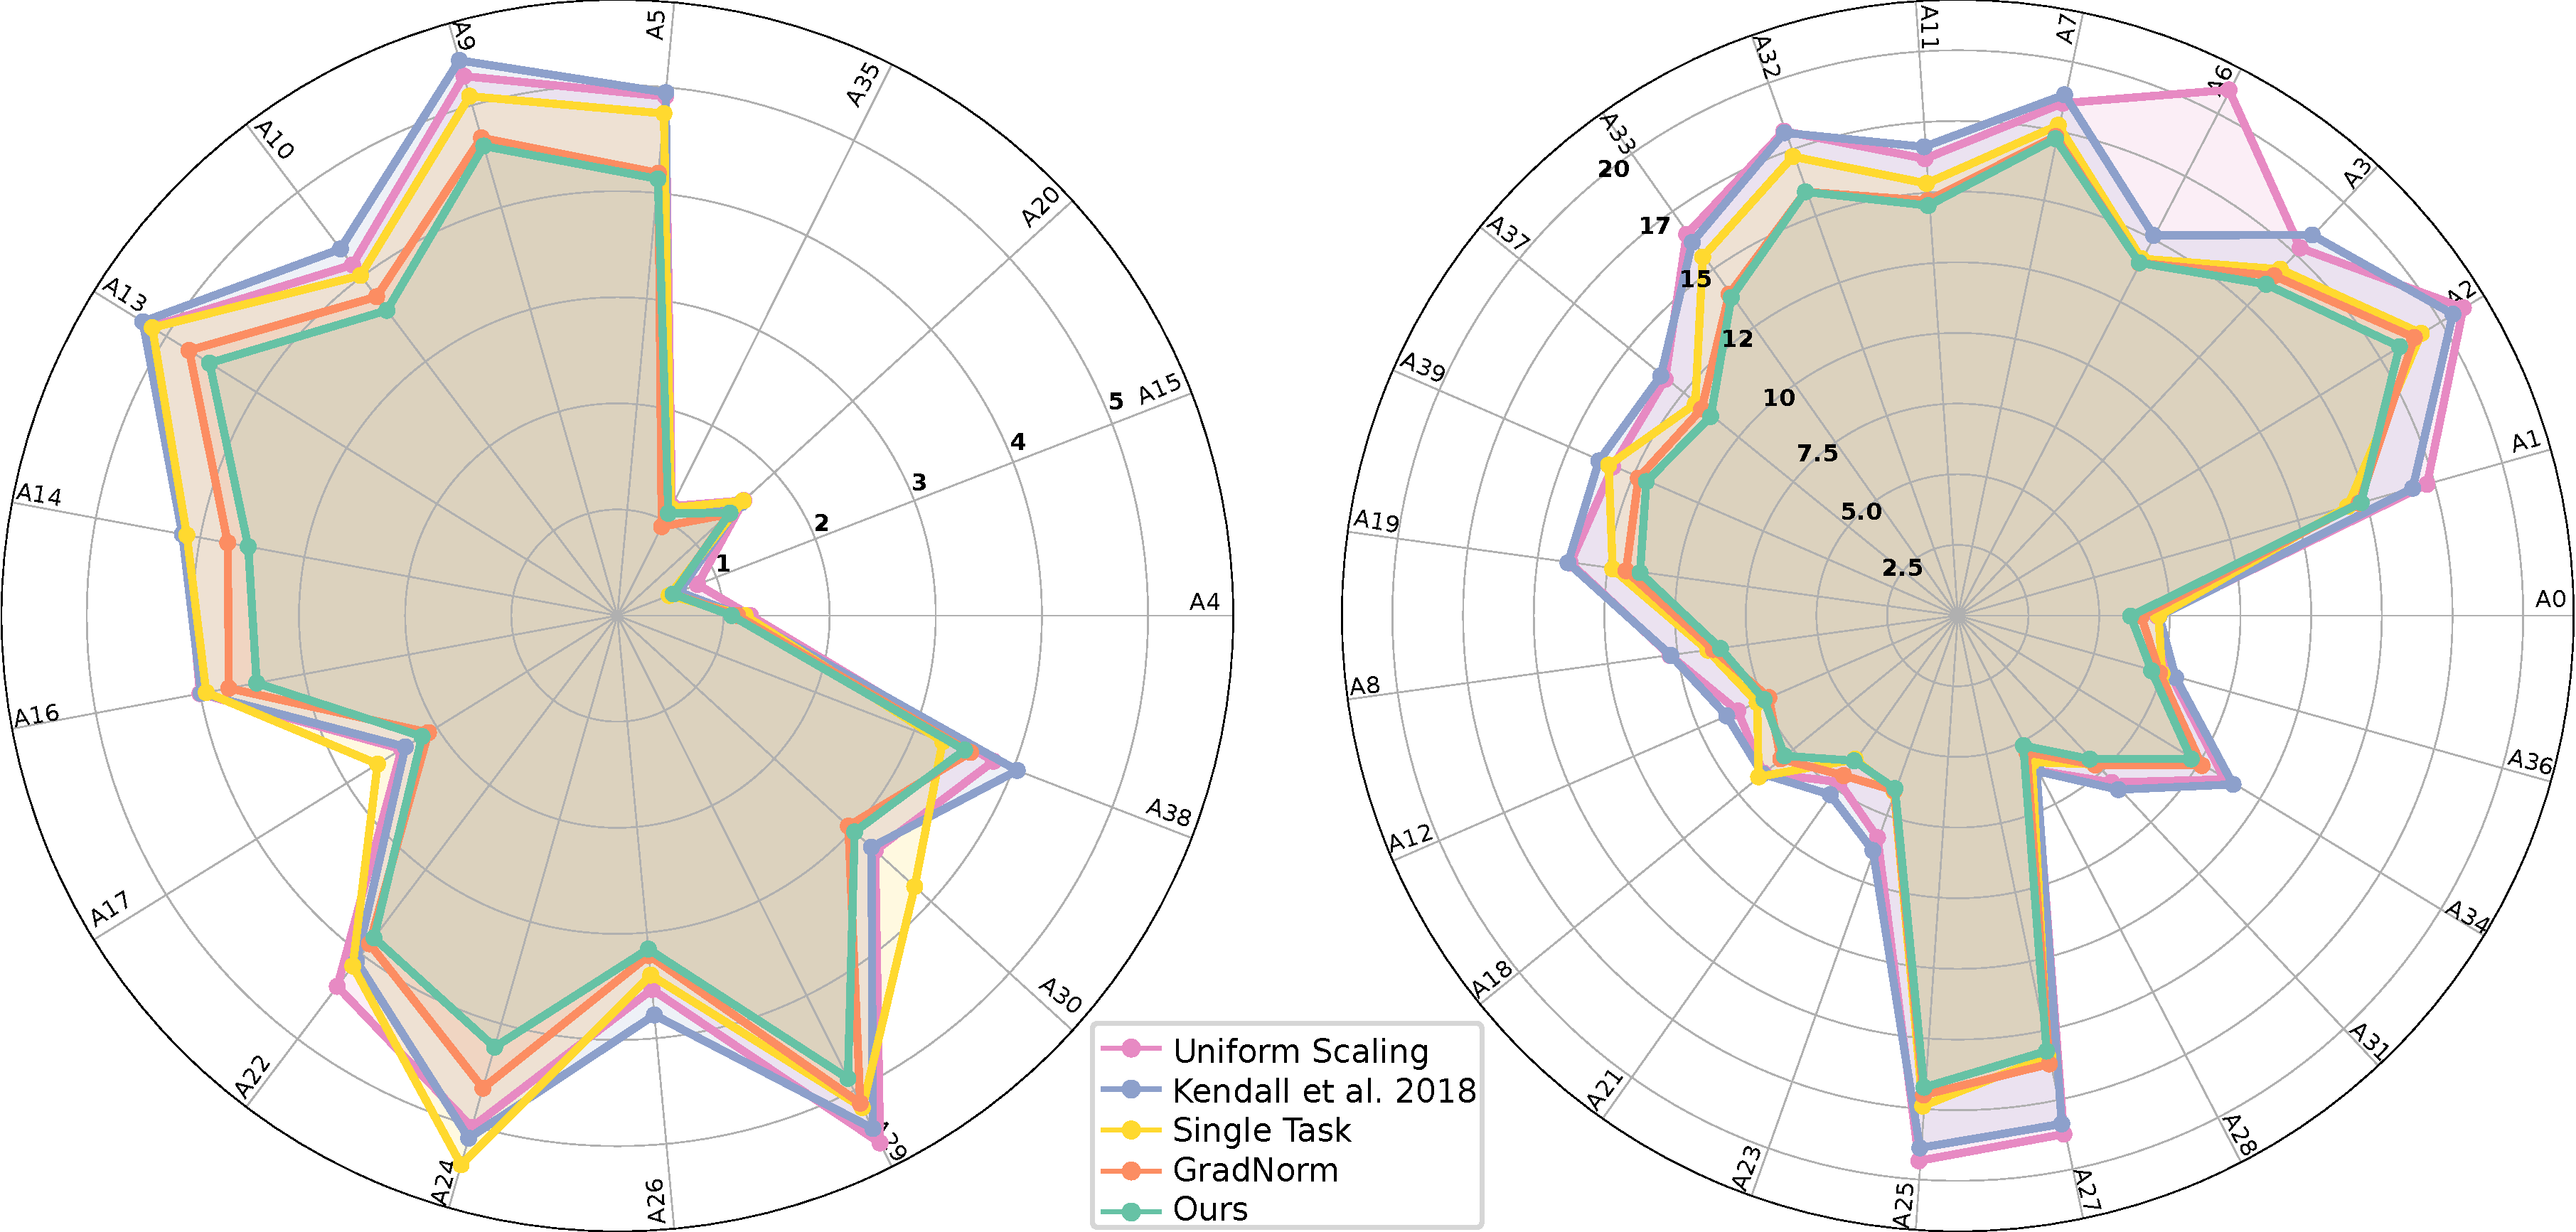
\includegraphics[width=\textwidth]{radar_full_new}
\vspace{1mm}
\caption{Radar charts of percentage error per attribute on CelebA \citep{celeba}. Lower is better. We divide attributes into two sets for legibility: easy on the left, hard on the right. Zoom in for details.}
\label{fig:multi_label_radar}
\end{figure}


\begin{wraptable}{r}{0.3\textwidth}
%\vspace{-4mm}
\captionof{table}{Mean of error per category of MTL algorithms in multi-label classification on CelebA \citep{celeba}.}
\begin{tabular}{r@{\hspace{2mm}}c@{}}
\toprule
& Average  \\
&  error \\
\midrule
Single task & $8.77$ \\
Uniform scaling & $9.62$ \\
\citealt{Kendall2018} & $9.53$ \\
GradNorm & $8.44$ \\
Ours & $\mathbf{8.25}$  \\
\bottomrule
\end{tabular}
\label{table:multi_label_bar}
%\vspace{-5mm}
\end{wraptable}

Next, we tackle multi-label classification. Given a set of attributes, multi-label classification calls for deciding whether each attribute holds for the input. We use the CelebA dataset \citep{celeba}, which includes 200K face images annotated with 40 attributes. Each attribute gives rise to a binary classification task and we cast this as a 40-way MTL problem. We use ResNet-18 \citep{resnet} without the final layer as a shared representation function, and attach a linear layer for each attribute (see the supplement for further details).


We plot the resulting error for each binary classification task as a radar chart in Figure~\ref{fig:multi_label_radar}. The average over them is listed in Table~\ref{table:multi_label_bar}. We skip grid search since it is not feasible over 40 tasks. Although uniform scaling is the norm in the multi-label classification literature, single-task performance is significantly better. Our method outperforms baselines for significant majority of tasks and achieves comparable performance in rest. This experiment also shows that our method remains effective when the number of tasks is high.


\subsection{Scene Understanding}

To evaluate our method in a more realistic setting, we use scene understanding. Given an RGB image, we solve three tasks: semantic segmentation (assigning pixel-level class labels), instance segmentation (assigning pixel-level instance labels), and monocular depth estimation (estimating continuous disparity per pixel). We follow the experimental procedure of \citet{Kendall2018} and use an encoder-decoder architecture. The encoder is based on ResNet-50 \citep{resnet} and is shared by all three tasks. The decoders are task-specific and are based on the pyramid pooling module \citep{pspnet} (see the supplement for further implementation details).

Since the output space of instance segmentation is unconstrained (the number of instances is not known in advance), we use a proxy problem as in \citet{Kendall2018}. For each pixel, we estimate the location of the center of mass of the instance that encompasses the pixel. These center votes can then be clustered to extract the instances. In our experiments, we directly report the MSE in the proxy task. Figure~\ref{fig:cityscapes_performance_profile} shows the performance profile for each pair of tasks, although we perform all experiments on all three tasks jointly. The pairwise performance profiles shown in Figure~\ref{fig:cityscapes_performance_profile} are simply 2D projections of the three-dimensional profile, presented this way for legibility. The results are also listed in Table~\ref{tab:cityscapes_results}.

MTL outperforms single-task accuracy, indicating that the tasks cooperate and help each other. Our method outperforms all baselines on all tasks.


\subsection{Role of the Approximation}

In order to understand the role of the approximation proposed in Section~\ref{sec:approximation}, we compare the final performance and training time of our algorithm with and without the presented approximation in Table~\ref{tab:approximation_tradeoff} (runtime measured on a single Titan Xp GPU). For a small number of tasks (3 for scene understanding), training time is reduced by 40\%. For the multi-label classification experiment (40 tasks), the presented approximation accelerates learning by a factor of 25.

On the accuracy side, we expect both methods to perform similarly as long as the full-rank assumption is satisfied. As expected, the accuracy of both methods is very similar. Somewhat surprisingly, our approximation results in slightly improved accuracy in all experiments. While counter-intuitive at first, we hypothesize that this is related to the use of SGD in the learning algorithm. Stability analysis in convex optimization suggests that if gradients are computed with an error $\hat{\nabla}_\btheta \mathcal{L}^t = \nabla_\btheta \mathcal{L}^t + \mathbf{e}^t$ ($\btheta$ corresponds to $\btheta^{sh}$ in (\ref{eq:kkt_opt})), as opposed to $\mathbf{Z}$ in the approximate problem in \ref{eq:approx}, the error in the solution is bounded as $\|\hat{\mathbf{\alpha}} - \mathbf{\alpha} \|_2 \leq \mathcal{O}(\max_t \|\mathbf{e}^t\|_2)$. Considering the fact that the gradients are computed over the full parameter set (millions of dimensions) for the original problem and over a smaller space for the approximation (batch size times representation which is in the thousands), the dimension of the error vector is significantly higher in the original problem. We expect the $l_2$ norm of such a random vector to depend on the dimension.

In summary, our quantitative analysis of the approximation suggests that (i) the approximation does not cause an accuracy drop and (ii) by solving an equivalent problem in a lower-dimensional space, our method achieves both better computational efficiency and higher stability.

  {\small
  \begin{table}[t]
%  \vspace{-4mm}
  \caption{Effect of the MGDA-UB approximation. We report the final accuracies as well as training times for our method with and without the approximation.}
  %\vspace{1mm}
  \centering
  \begin{tabular}{@{}r@{\hspace{3mm}}c@{\hspace{3mm}}c@{\hspace{2mm}}c@{\hspace{2mm}}c@{}c@{\hspace{5mm}}c@{\hspace{2mm}}c@{}}
  \toprule
  & \multicolumn{4}{c}{Scene understanding (3 tasks)} &  & \multicolumn{2}{c}{Multi-label (40 tasks)}  \\
  \cmidrule(r){2-5} \cmidrule(lr){7-8}
                  & Training & Segmentation & Instance  & Disparity      & & Training & Average \\
                 & time     &  mIoU [\%]       & error [px] & error [px] & & time (hour)      & error \\
  \midrule
  Ours (w/o approx.) & $38.6$ & $66.13$ & $10.28$ & $2.59$ & & $429.9$ & $8.33$ \\
  Ours & $\mathbf{23.3}$ & $\mathbf{66.63}$ & $\mathbf{10.25}$ & $\mathbf{2.54}$  & & $\mathbf{16.1}$ & $\mathbf{8.25}$ \\
  \bottomrule
  \end{tabular}
  %\vspace{-2mm}
  \label{tab:approximation_tradeoff}
  \end{table}}
